\subsection{Médiation des Appels Systèmes}
%% pourquoi: read/write, comm reseau 

Comme le montre la Figure \ref{AS_Communication}, les appels systèmes sont les
seules communications qui ne passent pas par un niveau d'abstraction. Ces
derniers communiquent directement avec le noyau. Le moyen le plus simple pour
intercepter les actions de l'application en gérant un minimum de choses semble
donc être l'interception des appels systèmes. Ces derniers sont constitués de
deux parties; l'entrée initialise l'appel via les registres de l'application qui
contiennent les arguments de l'appel puis donne la main au noyau. La sortie
inscrit la valeur de retour de l'appel système dans le registre de retour de
l'application, les registres d'arguments contenant toujours les valeurs reçues à
l'entrée de l'appel système, et rend la main à l'application. Nous devons donc
bloquer l'application à chaque interception d'une deux parties de l'appel
système. Ainsi, on pourra récupérer et modifier les informations permettant de
maintenir l'environnement simulé avant de rendre la main à l'application, pour
pouvoir entrer ou sortir de l'appel système.

 Dans cette section, nous allons présenter les outils existants qui permettent
 de faire cela.
 
 \subsubsection{L'appel système ptrace}
 \label{subsection:ptrace}
               
L'appel système \texttt{ptrace} \citep{AS:Interception, MARION:Interception},
dont la Figure \ref{PTRACE_FONCTIONNEMENT} illustre le fonctionnement, permet de
tracer tous les événement désirés d'un processus. Il peut également lire et
écrire directement dans l'espace d'adressage de ce dernier, à n'importe quel
moment ou lorsque un événement particulier se produit. De cette façon, on peut
contrôler l'exécution d'un processus. C'est un appel système dont chaque action
à effectuer est passée sous forme de requête en paramètre de l'appel système.

Pour pouvoir contrôler un processus via \texttt{ptrace}, on va créer deux
processus via un \texttt{fork}; un processus appelé ``processus espionné'' qui
exécutera l'application qu'on souhaite contrôler, et un autre qui contrôlera le
processus espionné, appelé ``processus espion''. Le processus espionné indiquera
au processus espion qu'il souhaite être contrôlé via un appel
système \texttt{ptrace} et une requête \texttt{PTRACE\_TRACEME} puis il
exécutera l'application via un \texttt{exec}. À la réception de cet appel, le
processus espion notifiera son attachement au processus espionné via un autre
appel à \texttt{ptrace} et une requête \texttt{PTRACE\_ATTACH}. Il indiquera
également sur quelles actions du processus espionné il veut être notifié (chaque
instruction, signal, sémaphore...), définissant ainsi les actions bloquantes
pour le processus espionné. Dans notre cas, ce seront les appels systèmes que
l'on considérera comme points d'arrêts (requête
\texttt{PTRACE\_SYSCALL)}. Ainsi, le processus espion sera donc appelé deux
fois: à l'entrée et à la sortie de chaque appel système.

Quand un processus de l'application voudra faire un appel système, il sera
bloqué avant de l'exécuter et le processus espion qui lui est associé sera
notifié. Ce dernier effectue alors les modifications nécessaires dans les
registres du processus espionné pour conserver la virtualisation de
l'environnement. Ensuite, il rendra la main au processus espionné pour que
l'appel système puisse avoir lieu. Le même fonctionnement est utilisé pour le
retour de l'appel système. Le processus espion change simplement le temps
d'exécution de l'appel système et l'horloge de l'application en utilisant ceux
calculés par le simulateur. Quand un processus espion a fini un suivi, il peut
envoyer deux types de requêtes au processus espionné: \texttt{PTRACE\_KILL} qui
termine le processus espionné ou \texttt{PTRACE\_DETACH} qui le laisse continuer
son exécution.

\begin{figure}
\centering
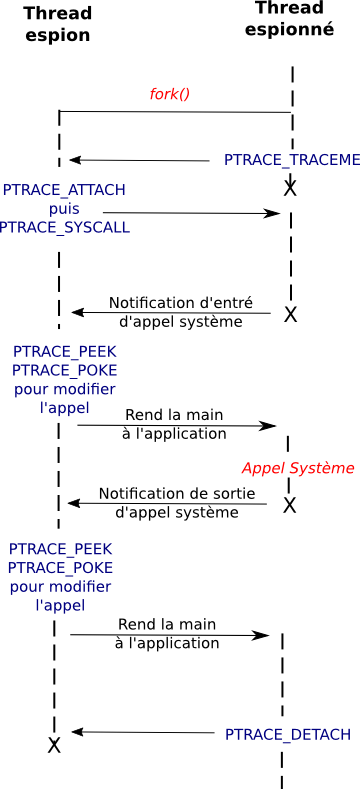
\includegraphics[scale=0.5]{Pictures/png/ptrace_fonctionnement}
\caption{Attachement d'un processus et contrôle via un espion}
\label{PTRACE_FONCTIONNEMENT}
\end{figure}

Néanmoins, pour contrôler un processus, \texttt{ptrace} fait de nombreux
changements de contexte pour pouvoir intercepter et gérer les événements, or
cela coûte plusieurs centaines de cycles CPU. De plus, il supporte mal
les processus utilisant du multithreading, et ne fait pas partie de la norme
POSIX. Ainsi il peut ne pas être disponible sur certaines architectures et son
exécution peut varier d'une machine à une autre.

Nous tenons à faire remarquer que l'utilitaire UNIX \texttt{strace}\footnote{\url{http://linux.die.net/man/1/strace}} suit la même approche que \texttt{ptrace} sans avoir ses désavantages, mais qu'il a été écarté car il ne fait qu'afficher les appels systèmes réalisés par une application.

%% Non module noyau
\subsubsection{Uprobes}

Uprobes \citep{AS:Interception, MARION:Interception}, pour \textit{user-space
  probes}, est une API noyau permettant d'insérer dynamiquement des points
d'arrêts à n'importe quel endroit dans le code d'une application et à n'importe
quel moment de son exécution. Nous pouvons donc l'utiliser avec les appels
systèmes comme points d'arrêts.

La façon la plus classique d'utiliser cette interface se base sur Utrace,
équivalent de \texttt{ptrace} en mode noyau. Ce dernier permet d'éviter les
nombreux changements de contexte, qui dégradent les performances, et offre une
meilleure gestion du multithreading. Dans cette version, l'utilisateur fournit
pour chaque point d'arrêts un handler particulier à exécuter avant ou après
l’instruction marquée. Uprobes étant un outil s'exécutant dans le noyau, les
handlers doivent être placés dans un module noyau. Ce dernier contient pour
chaque point d'arrêt géré par Uprobes le handler à exécuter, ainsi que le pid du
processus concerné et l'adresse virtuelle du point d'arrêt. Pour gérer un point
d'arrêt Uprobes utilise trois structures de
données \textit{i)} \texttt{uprobe\_process} (une par processus controlé),
\textit{ii)} \texttt{uprobe\_task} (autant que le processus contrôlé a de
threads), \textit{iii)} \texttt{uprobe\_kimg} (une pour chaque point d'arrêt
affectant un procesus). Chaque structure \texttt{uprobe\_task} et
\texttt{uprobe\_kimg} sont propres à une structure \texttt{uprobe\_process}. La
fonction \texttt{init} du module va poser les points d'arrêt et la fonction
\texttt{exit} les enlevera. Pour cela, on utilise respectivement la fonction
\texttt{register\_uprobe} et \texttt{unregister\_uprobe}. Ces deux fonctions ont
pour argument le pid du processus à contrôler, l'adresse virtuelle du point
d'arrêt dans le code et le handler à exécuter quand le point d'arrêt est
atteint. La fonction \texttt{register\_uprobes} va trouver le processus passé en
paramètres en parcourant la liste des structures \texttt{uprobes\_process} ou la
crééra si cette dernière n'existe pas. Ensuite, elle crée la structure
\texttt{uprobe\_kimg}, puis fait appel à Utrace pour bloquer l'application, le
temps de placer le point d'arrêt dans le code de celle-ci. Pour cela, on va
insère avant l'instruction sondée un appel au module contenant le handler à
invoquer, puis on rend la main à l'application en utilisant de nouveau
Utrace. \texttt{unregister\_uprobe} fait de même mais supprime la structure
\texttt{uprobe\_kimg} passée en paramètre au lieu de l'ajouter. De plus, s'il
s'agit de la dernière structure de ce type pour un processus contrôlé, il
supprimera alors la structure \texttt{uprobe\_process} et toutes les
\texttt{uprobe\_task} associées.

Lorsqu'un point d'arrêt est atteint Uprobes prend la main et exécute le handler
correspondant. Pour savoir qu'un point d'arrêt a été atteint, Uprobes utilise de
nouveau Utrace, ce dernier envoyant un signal à Uprobes à chaque fois que le
processus qu'il contrôle atteint un point d'arrêt.

Utrace envoie également un signal à Uprobes quand un des processus contrôlé fait
un appel à \texttt{fork}, \texttt{clone}, \texttt{exec}, \texttt{exit} pour que
ce dernier créé ou supprime les structures \texttt{uprobe\_process}
concernées. Utrace peut également être utilisé dans le handler gérant un point
d'arrêt pour récupérer des informations sur l'application et les données qu'elle
utilise. De plus, un handler peut également ajouter ou enlever des points
d'arrêts.

Les deux avantages de cette solution sont qu'elle est rapide et qu'elle a accès
à toutes les ressources sans aucune restriction.

\subsubsection{Seccomp/BPF}
%% Read only
\label{paragraph:seccomp/bpf}

\texttt{seccomp}\footnote{Seccomp man \url{http://man7.org/linux/man-pages/man2/seccomp.2.html}} est un appel système qui permet d'isoler un processus
en lui donnant le droit de n'appeler et de n'exécuter qu'un certain nombre d'appels
systèmes: \texttt{read}, \texttt{write}, \texttt{exit} et \texttt{sigreturn}. Si
le processus fait un autre appel système, il sera arrêté avec un signal
\texttt{SIGKILL}. Comme cela est assez contraignant, le nombre d'applications
que l'on peut utiliser avec \texttt{seccomp} est donc limité. Pour plus de
flexibilité, on peut utiliser une extension de cet appel système appelée
seccomp/BPF, pour \textit{seccomp BSD Packet Filter}, permettant de définir dans
un programme BPF \citep{BPF_mccanne1993bsd} les appels systèmes autorisés à
s'exécuter, en plus de ceux cités précédemment. Cette extension fonctionne sur le
même principe que le filtrage de paquet réseau où on établit une suite de
règles. Pour pouvoir s'exécuter, un appel système doit pouvoir passer à travers
toutes les règles. Dans le cas où les appels systèmes \texttt{fork} ou
\texttt{clone} peuvent s'exécuter, l'arborescence de filtres est transmise aux
enfants, de même que pour les processus faisant des appels \texttt{execve}
quand ils sont autorisés. Les règles des filtres BPF portent sur le type de
l'appel système et/ou ses arguments. Ainsi, à chaque entrée ou sortie d'un appel
système, ne faisant pas partie des quatre autorisés par \texttt{seccomp}, l'extension
utilisant BPF est appelée. Elle reçoit en entrée le numéro de l'appel système,
ses arguments et le pointeur de l'instruction concernée. En fonction des règles,
elle laisse l'appel système s'exécuter ou pas.  De plus, seccomp/BPF possède une
option qui lui permet de générer un appel système \texttt{ptrace}. Cela permet
au processus espion, s'il existe, de ne plus attendre sur chaque appel système
du processus espionné, mais uniquement sur les appels systèmes qu'il souhaite
intercepter.

L'appel système seccomp et son extension seccomp/BPF sont disponibles uniquement si
le noyau est configuré avec l'option \texttt{CONFIG\_SECCOMP} pour la première
et \texttt{CONFIG\_SECCOMP\_FILTER} pour la seconde. Pour pouvoir créer des
filtres, il faut également avoir des droits particuliers, notamment l'exécution
de certaines commandes administrateurs. Ainsi, l'utilisation de cet appel
système et de son extension demande une certaine configuration noyau et des
privilèges pour les utilisateurs.

De plus, si on l'utilise sans l'option d'appel à \texttt{ptrace}, on ne peut que
lire le contenu de l'appel système et pas le modifier. On ne peut donc pas faire
de médiation avec cet outil sans faire appel à \texttt{ptrace}. Néanmoins,
l'utilisation de seccomp/BPF avec \texttt{ptrace} permet de réduire
signifiquativement le nombre d'événements sur lequel attendra le processus
espion.

